%% 
%% Copyright 2007-2020 Elsevier Ltd
%% 
%% This file is part of the 'Elsarticle Bundle'.
%% ---------------------------------------------
%% 
%% It may be distributed under the conditions of the LaTeX Project Public
%% License, either version 1.2 of this license or (at your option) any
%% later version.  The latest version of this license is in
%%    http://www.latex-project.org/lppl.txt
%% and version 1.2 or later is part of all distributions of LaTeX
%% version 1999/12/01 or later.
%% 
%% The list of all files belonging to the 'Elsarticle Bundle' is
%% given in the file `manifest.txt'.
%% 

%% Template article for Elsevier's document class `elsarticle'
%% with numbered style bibliographic references
%% SP 2008/03/01
%%
%% 
%%
%% $Id: elsarticle-template-num.tex 190 2020-11-23 11:12:32Z rishi $
%%
%%
\documentclass[review,3p]{elsarticle}

%% Use the option review to obtain double line spacing
%% \documentclass[authoryear,preprint,review,12pt]{elsarticle}

%% Use the options 1p,twocolumn; 3p; 3p,twocolumn; 5p; or 5p,twocolumn
%% for a journal layout:
%% \documentclass[final,1p,times]{elsarticle}
%% \documentclass[final,1p,times,twocolumn]{elsarticle}
%% \documentclass[final,3p,times]{elsarticle}
%% \documentclass[final,3p,times,twocolumn]{elsarticle}
%% \documentclass[final,5p,times]{elsarticle}
%% \documentclass[final,5p,times,twocolumn]{elsarticle}

%% For including figures, graphicx.sty has been loaded in
%% elsarticle.cls. If you prefer to use the old commands
%% please give \usepackage{epsfig}

%% The amssymb package provides various useful mathematical symbols
\usepackage{amssymb}
%% The amsthm package provides extended theorem environments
\usepackage{amsthm}
\usepackage{subcaption}
\usepackage[T1]{fontenc}
\usepackage{babel}
%% The lineno packages adds line numbers. Start line numbering with
%% \begin{linenumbers}, end it with \end{linenumbers}. Or switch it on
%% for the whole article with \linenumbers.
\usepackage{lineno}

\journal{Journal of Quantitative Spectroscopy $\&$ Radiative Transfer}

\begin{document}

\begin{frontmatter}

%% Title, authors and addresses

%% use the tnoteref command within \title for footnotes;
%% use the tnotetext command for theassociated footnote;
%% use the fnref command within \author or \address for footnotes;
%% use the fntext command for theassociated footnote;
%% use the corref command within \author for corresponding author footnotes;
%% use the cortext command for theassociated footnote;
%% use the ead command for the email address,
%% and the form \ead[url] for the home page:
%% \title{Title\tnoteref{label1}}
%% \tnotetext[label1]{}
%% \author{Name\corref{cor1}\fnref{label2}}
%% \ead{email address}
%% \ead[url]{home page}
%% \fntext[label2]{}
%% \cortext[cor1]{}
%% \affiliation{organization={},
%%             addressline={},
%%             city={},
%%             postcode={},
%%             state={},
%%             country={}}
%% \fntext[label3]{}

\title{Investigating the applications and limits of single particle light scattering using limited detection schemes}

%% use optional labels to link authors explicitly to addresses:
%% \author[label1,label2]{}
%% \affiliation[label1]{organization={},
%%             addressline={},
%%             city={},
%%             postcode={},
%%             state={},
%%             country={}}
%%
%% \affiliation[label2]{organization={},
%%             addressline={},
%%             city={},
%%             postcode={},
%%             state={},
%%             country={}}

\author[aff1]{Dan Maciver}
\affiliation[aff1]{organization={Department of Chemical Engineering,
			University of Strathclyde},
            addressline={16 Richmond Street}, 
            city={Glasgow},
            postcode={G1 1XQ}, 
            country={Scotland}}
\author[aff1]{Praveen Parthasarathi}
\author[aff1]{Mark Haw}
\author[aff1]{Leo Lue}
\author[aff1]{Jan Sefcik}

\begin{abstract}
Combing light scattering techniques with optical trapping set ups poses a significant engineering challenge. We propose a optical tweezer set up that will allow for light scattering measurements of a trapped micro particle. The set up is constrained by the limited space available to place optical fibres within range of the trapped entity. This paper discusses how light scattering data from a trapped dimer can be used to predict the orientation of the dimer within the trap. This method can be extended for determining characteristics that influence the light scattering pattern. We also discuss the how to determine best possible arrangement of optical fibres that will provide the greatest accuracy in our prediction. We hope to take this work further with real experimental data from our own light scattering measurements. 

\end{abstract}

%%Graphical abstract
\begin{graphicalabstract}
	\centering
	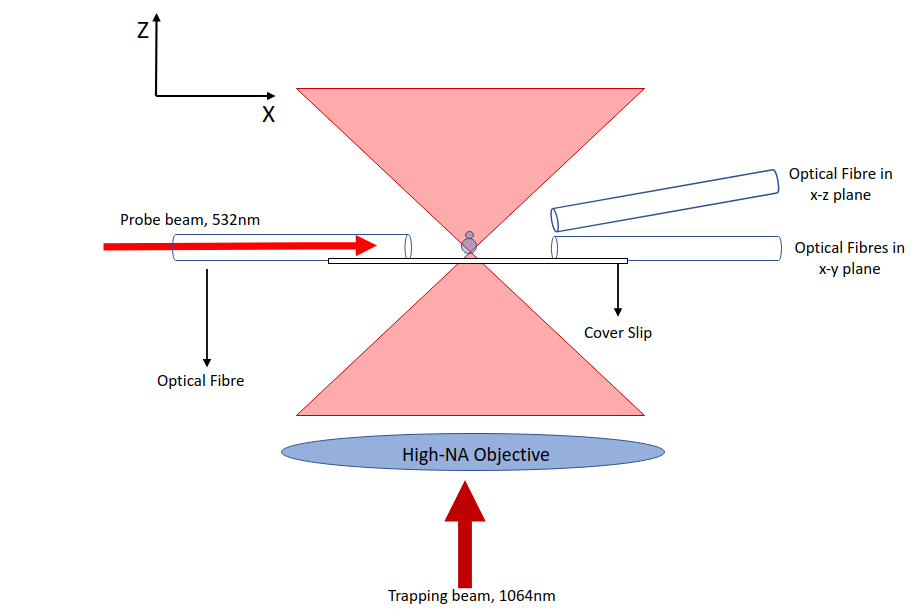
\includegraphics[width=0.8\textwidth, height = 0.6\textheight]{fig1a.png}
\end{graphicalabstract}

%%Research highlights
\begin{highlights}
\item Asymmetric dimers of undergo a full inversion in the presence of an potential well
\item Orientation can be classified by applying Bayesian Statistics to light intensity readings
\item Bayesian model shows increased accuracy when processing noisy signal measurements. 
\item Multiple estimations can be  used to cancels out artefacts of noise. 
\end{highlights}

\begin{keyword}
	Optical Trapping \sep Light Scattering \sep Measurements \sep Statistics

\end{keyword}

\end{frontmatter}

%%\linenumbers

%% main text
\section{Introduction}
\label{1}

Since their invention in the late 1980's, Optical Tweezers have found application in experiments ranging from single molecule biophysics~\cite{Wang 2021} to those that test the fundamental assumptions of Quantum Mechanics ~\cite{Duan 2013} thanks mainly to the ability of the tweezer to transduce and detect forces in the order of a few pico-newton. Recent applications of the Optical Tweezers in metrological measurements ~\cite{Scott Waitukaitis} and colloidal aggregation ~\cite{Optical Binding} demand the tweezer to also be able to characterise  the trapped entity. To this end, chemical characterisation of the trapped entities has been achieved using spectroscopic techniques such as Raman Scattering ~\cite{P K Gupta} and dynamical characterisation has been achieved mainly by following the centre-of-mass Brownian motion of the trapped entity using a Quadrant Photo Detector~\cite{Alexander Rohrbach}. While this technique has allowed for detection of linear motion of trapped entities  with sub-nanometre precision~\cite{Alexander Rohrbach} and  rotation~\cite{recent paper} of the centre-of-mass, there is a paucity of literature on measuring the orientation of trapped non-spherical particles till the recent attempt in ~\cite{New Zealand paper} where imaging was employed to study the orientation of trapped dimers and a resolution of () was achieved.   

Possibility of integrating light scattering with optical trapping was demonstrated by Bar-Ziv et.al.,~\cite{Bar-Ziv_1998} where a single-mode optical fibre was aligned to detect the scattered light from a trapped bead and it's Brownian motion was studied. While this allowed for studying the dynamics, any information with regards structure of the trapped bead was precluded as the measurement was a single-angle scattering measurement.
In this work, we propose a novel Bayesian Inference based technique to interpret light scattering data detected in a scheme that expands on the technique in ~\cite{Bar-Ziv_1998} to detect scattered light simultaneously at 3 angles as shown in Figure 1.

\section{Theory}
\label{2}

Consider a dimer with unequal sphere diameters $a_1, a_2$ in an optical trap positioned in some orientation $\hat{s}$. Due to the Brownian motion from the surrounding fluid the dimer's orientation changes with time. Assuming we cannot accurately determine the dimer's orientation from imaging alone we instead rely on it's light scattering. We collect the near field intensity, via optical fibres,from a probe laser at 3 predetermined angles $\theta_1, \theta_2, \theta_3$. To determine the particle's orientation we compare the produced light scattering signal to a collection of reference orientations that are evenly spaced around the orientation space.

\begin{figure}[t]
	\centering
	\includegraphics[width = 0.5\textwidth]{junk_00078.png}
	\caption{Reference orientations plotted in the physical space. Green arrow points in the direction of the dimers orientation. The red point is our estimation, and the green point is the best possible estimate.}
\end{figure}

We use the a Fortran package specialised for calculating non spherical t-matrices (MSTM) \cite{MSTM} to determine the light scattering intensity of our dimer in each reference orientation. We assume that the for each detection fibre the intensities can be distributed on a Gaussian curve centred at $y_k$, the normalised intensity at detection fibre k. Based on the light scattering from the dimer we can assign a probability that the produced light scattering pattern produced belongs to the reference orientation $\hat{n}$

	\begin{eqnarray}
		p(y(\hat{s})\parallel\hat{n})&= \Pi^3_{k=1} 
		(2\pi\sigma_k^2)^{-1/2} e^{-(y(\hat{n})_k-y(\hat{s})_k)^2/2\sigma_k^2}
	\end{eqnarray}

Where $\sigma_k$ is the average error in our signal collection; we left this as a tuneable variable to measure how the influence of experimental error would effect our predictive model. This was implemented by adjusting the values of $y(\hat{s}_k)$. 
\begin{eqnarray}
	\sigma_k = 0.17\bar{y}(\hat{n}_k) \\
	\Rightarrow y(\hat{s}_k) = y(\hat{s})_k \pm n\sigma_k \\ 
	n \in \mathbb{R}, n\in[0,1]
\end{eqnarray}

We can view this result as a conditional probability, if the orientation is determined ($\hat{n}$) then what is the probability that expected scattering signal matches our dimer's scattering signal. We instead want to know the inverse conditional, that with a given signal y the dimer was in orientation $\hat{n}$. We can calculate this using Bayes' theory:

\begin{eqnarray}
	p(\hat{n}\parallel y(\hat{s}))&= \frac{p(y(\hat{s})\parallel\hat{n})p(\hat{n})}{p(y)}
\end{eqnarray}

Where $p(\hat{n})$ and $p(y)$ are our estimations of the priori distributions of particle orientations and scattering signals respectively. The former can be estimated by some Boltzmann distribution based on the spacing between reference orientations. The latter priori $p(y)$ is the probability of our dimer producing the signal $y$ and is given as. 

\begin{eqnarray}
	p(y) = \int p(y(\hat{s})\parallel \hat{n}) p(\hat{n}) d\hat{n}
\end{eqnarray}
In order to test the accuracy of our model we first test it using an idealised simulation of the target dimer. 

\subsection{Testing the model}
\label{2.1}
We use the Brownian OT package by Jerome Fung \cite{Brownian_OT} to simulate how our target dimer moves while subject to an optical trap. At each time step we determine the dimer's orientation and use MSTM to calculate its scattering pattern. We then use the above method to estimate the dimer orientation based on its scattering pattern. The priori estimate $p(\hat{n})$ can be defined as a Boltzmann's distribution based on the dot product of our previous estimation $\hat{n}_{t-\Delta t}$ and each reference orientation $\hat{n}_t$:
\begin{eqnarray}
	r_j(t, \hat{n})= \hat{n}_{t} \cdot \hat{n}_{t-\Delta t} \\
	p(\hat{n})= \frac{e^{(r_j(t,\hat{n})-1)}}
	{\Sigma_{i=1}^{24}e^{r_i(t, \hat{n})}}
\end{eqnarray}

Since we are testing with a simulation we already know the exact orientation of the dimer, we want to know how often our model can determine the closest reference orientation $\hat{n}$ to the true orientation $\hat{s}$, and how precise our prediction is. For a perfect model our probability distribution should equal 1 at the correct result and zero elsewhere. In reality our model will be some probability distribution that has some probability of any orientation being correct. To evaluate our model's accuracy and confidence we calculate the Kullback-Leibler divergence of the two probability distributions. 

\begin{eqnarray}
	K_{l, \#}(p_{guess} \parallel p_{ideal}) &= 
	p_{ideal} \ln \left[
	\frac{p_{ideal}}{p(\hat{n}\parallel y_k(\hat{s}))}
	\right]
\end{eqnarray}

Where the divergence goes to zero if $p_{ideal}=0$, for a single estimation this gives us an idea of both how confident our model is in it's estimation. We sum the divergence of each measurement across the entire simulation to get an idea of how well the model performs across the entire simulation. To measure how much our result had improved we compare it to a worse case scenario, where every $\hat{n}$ is given uniform probability, and evaluate the improvement factor $F(K_l)$

\begin{eqnarray}
	K_{l,total} = \sum\limits_{\# =1}^{timesteps} K_{l,\#} \\
	F(K_l) = \frac{K_{l,\ worst}}{K_{l,total}}
\end{eqnarray}

To measure how much our result had improved we compare it to a worse case scenario, where every $\hat{n}$ is given uniform probability. Since our divergence result is a product of our choice of angles we can see analyse how the choice of angles can be altered to improve our estimate.  

\subparagraph{Optimization of angle choice}
\label{2.2}
The efficacy of our estimation is a function of our detection angles, testing every possible configuration manually is time consuming, therefore we utilised Ultra nest to apply a Monte Carlo simulation to our model. Ultra-nest is a sophisticated python package for fitting models with complex parameter interactions \cite{Ultranest}. Ultra-nest implements a variation of Monte Carlo integration,nested-sampling, where the likelihood contour is used to update a group of live points chosen from the prior estimation.

We used the Ultra-nest software to create a set of live points of different choices of $\theta_1, \theta_2, \ \& \ \theta_3$, with each point being evaluated by the divergence ($K_{l, total}$) produced. After evaluating every live point, the worst results are removed and new live points are created based on the information provided by the previous live points. This results in a convergence on parameter choices that result in an average divergence result of almost 0. A common issue with complex parameter spaces, such as ours, is the issue of degeneracies (where two or more parameters have identical parameter spaces), to combat this we implemented a random step sampler that selects a new live point some 'n' steps away in the parameter space.
 
\section{Results}
\label{3}
\subsection{Asymmetric dimer dynamics}
\label{3.1}
The Brownian OT software was used to simulate the motion of a trapped dimer ($a_1=1\mu m, a_2=0.5\mu m$) over the first 10 seconds of entering the optical trap. The initial orientation was assumed as strictly vertical (in line with the beam propagation direction). The dimer's position orientation was recorded every $10 \mu s$ for using as a test dataset for our model. 

\begin{figure}[h]
	\centering
	\begin{subfigure}{0.45\textwidth}
		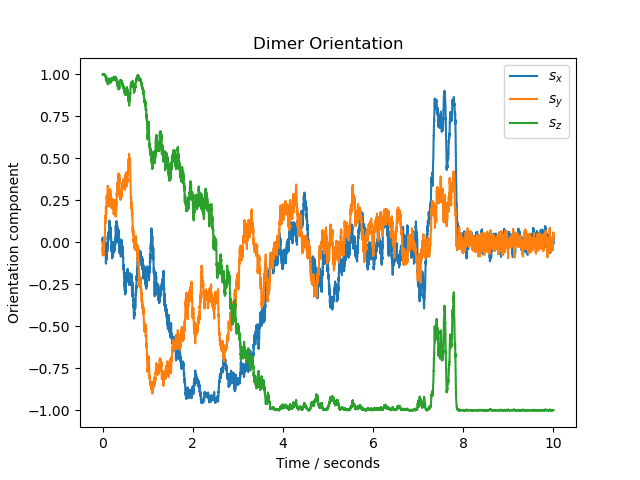
\includegraphics[width =\textwidth]{traj.png}
	\end{subfigure}
	\begin{subfigure}{0.45\textwidth}
		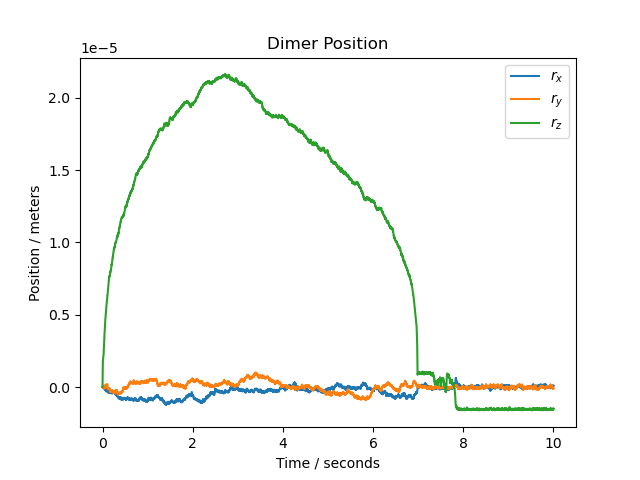
\includegraphics[width=\textwidth]{pos.png}
	\end{subfigure}
	\caption{Simulation results of: a) the dimers orientation vector with time, b) the dimer's [x,y,z] position with time.}
\end{figure}

As can be seen from \figurename{ 2}, the dimer undergoes a full $180^{\circ}$ rotation upon entering the trap. Typically horizontal alignment of a dimer is unstable and will result in the particle rotating to align along its vertical axis. It is interesting to note that the dimer is furthest from the trap centre as it goes into a horizontal orientation before drawing closer again as it inverts completely. Further simulations of differently sized dimers showed similar results, but only when $a_1 \geq 2a_2$. Dimers with more symmetrical size ratios immediately aligned into a fixed vertical position. 
In Vigilante's work with dimers \cite{Brownian_OT} simulations of trapped symmetrical dimers was investigated; their findings showed that the optical torque on the dimer goes to zero while aligned vertically and is at its maximum in a horizontal alignment. Therefore, the inversion of an asymmetric dimer suggests that if the size difference is significant the optical torque goes is minimal for a dimer in both horizontal and vertical orientations. Once we have our experimental set up complete we can confirm this by trapping an asymmetric dimer and monitoring its orientation. 

\subsection{Predictive efficacy of model}
\label{3.2}
The data from \figurename{ 2a} was used to test the efficacy of our predictive model. To visualise how well our model tracks the dimer's orientation we plot the radial distance between our model's prediction and the true orientation, and between the best possible orientation and the true orientation. For a perfect estimation these two plots should overlap. 

We first tested how varying the error value would effect our model's efficacy; calculating the improvement factor $F(K_l)$ with each test. As can be seen from \figurename{ 3} our model actually performs better with noisy signals, to the extent that a signal error of $10\%$ resulted in a worse performance than if we had just guessed each orientation at random. 
\begin{figure}
	\begin{subfigure}{0.33\textwidth}
		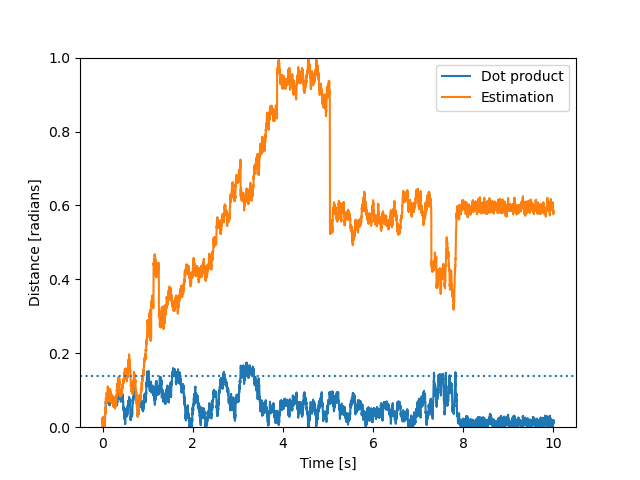
\includegraphics[width=\textwidth]{Error_10_percent.png}
		\subcaption{$F(K_l) = 0.9422$}
	\end{subfigure}
	\begin{subfigure}{0.33\textwidth}
		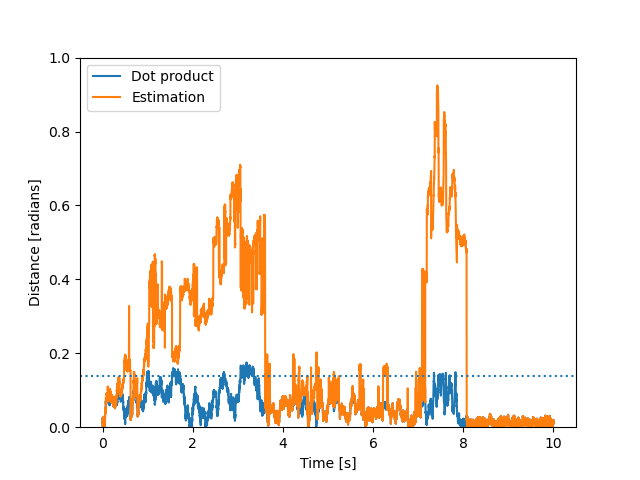
\includegraphics[width=\textwidth]{Error_20_percent.png}
		\subcaption{$F(K_l) = 1.366$}
	\end{subfigure}
	\begin{subfigure}{0.33\textwidth}
		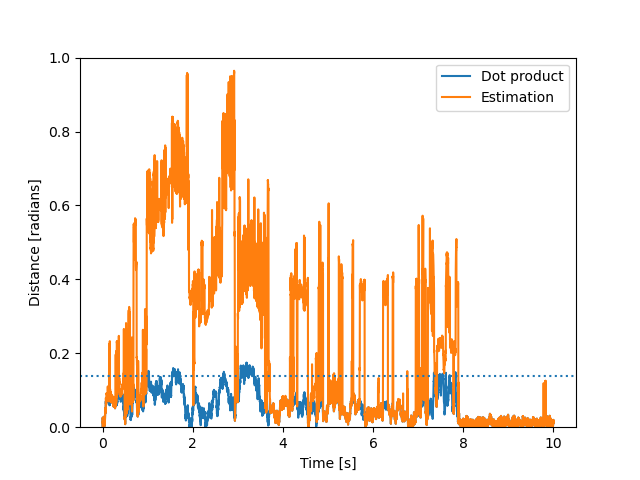
\includegraphics[width=\textwidth]{Error_30_percent.png}
		\subcaption{$F(K_l)=1.440$}
	\end{subfigure}
	\caption{Model predictions with signal error at a) $10 \%$, b)  $20\%$, and c) $30\%$}
\end{figure}

The issue with having a high signal error is that our model's prediction can be very far off from the correct answer and still be confident with it's results; fortunately our priori for the dimer's orientation can help to correct our estimate by limiting the probability in the physical space. We found that the inclusion of our priori estimate compared to a uniform priori improved our results by around $20 \%$. We can alter the influence of our priori by adding an additional exponential 

\subsection{Ultra-nest results}
\label{3.3}
We first allowed ultra nest to traverse the parameter space while each angle was constrained to a predefined area. We assumed that the each fibre would be placed within a roughly $30^{\circ}$ range so that we get a sampling of the entire light scattering pattern, we didn't search further than $100^{\circ}$ as the signals would be to low to detect for a micron scale scatterer. The sampler ran until the divergence result was in the order of $10^1$.

\begin{figure} [t]
	\centering
	\includegraphics[width=0.4\textwidth]{Cornerangleconstrained-1.png}
	\caption{Corner plot from ultra-nest, darker regions indicate a better divergence result. $\theta_1$ was constrained between $15^{\circ}$ and $25^{\circ}$; $\theta_2$ was constrained between $30^{\circ}$ and $60^{\circ}$; $\theta_3$ was constrained between $65^{\circ}$ and $100^{\circ}$.}
\end{figure}
As can be seen from \figurename{ 4} the parameter space for our angle choice is essentially flat, with no explicit maxima to be found, the sudden increase in our divergence around $\theta_1 = 18^{\circ}$ is likely due to the fact that if we consider the scattering curves for our reference orientations there exist local minima on at roughly $\theta_1 = 13^{\circ}$ and $25^{\circ}$. Therefore between these two minima the model struggles to differentiate between reference orientations given that the light intensity is similar for different orientations. 

We then decided to remove the limitations on our choice of angles, the only constraining factor being that the fibre's could not be placed within $10^{\circ}$ of each other. 

\begin{figure} [h]
	\centering
	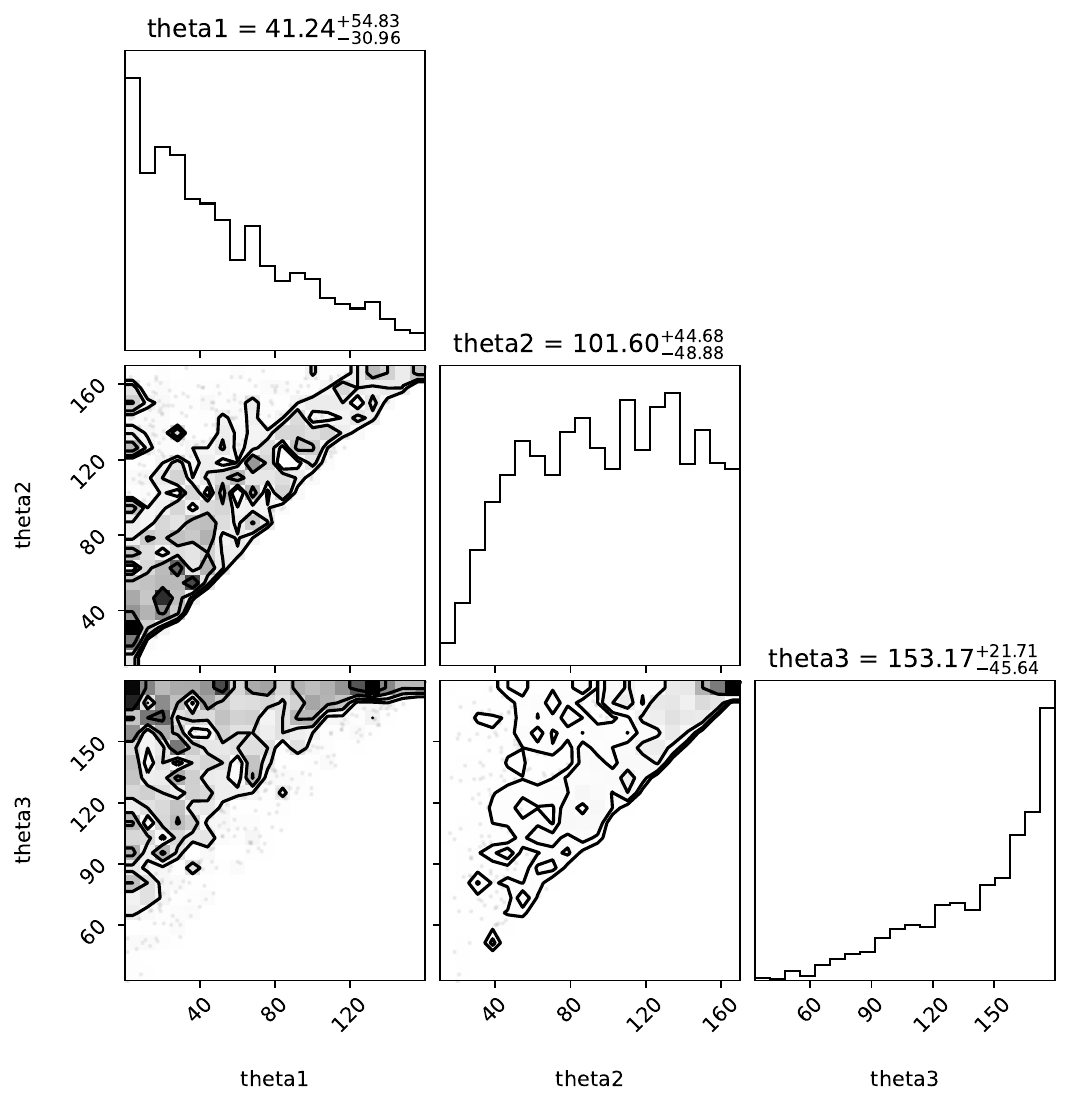
\includegraphics[width=0.4\textwidth]{corneranglesfreed-1.png}
	\caption{Corner plot from ultra-nest, darker regions indicate a better divergence result. Choice of angles is not limited to a predefined region.}
\end{figure}

Now we see that allowing the angles to be anywhere in the parameter space results in a more focused result for both $\theta_2$ and $\theta_3$ but still a flat parameter space for $\theta_1$. The result suggests that the model is more successful when we allow for backscattering to be considered in our model. While this works for a perfect system where noise is a known quantity it is unlikely if the signals are clear enough under laboratory conditions.

	
\section{Conclusion}
\label{4}
We have developed a model for interpreting the dynamics of a trapped particle based purely on the light scattering pattern. Compared to a random selection of the particle's orientation we find that our model has a $150\%$ increase in it's accuracy. Even more interestingly, our model performs better under noisy signal conditions by allowing our estimate to self-correct itself, in the future we hope to remove the artefacts of the signal noise by combing multiple estimates using different detection angles. This can be achieved via the inclusion of additional signal detections, we refrained from collecting more signal point for two key reasons; firstly, we wanted to show the extent of the mathematical model in the case of limited detection schemes, and secondly, we wanted to limit our model to what is possible in a real world experimental set up. Once we have a clearer understanding of the maximum limit of detection fibres that can be placed we can update our model to account for this and improve the accuracy further. 

Our simulations of asymmetric dimers found that for large sphere ratios the dimer will prefer to be orientated against the beam propagation and will even move further from the trapping focus to invert itself before coming back to the laser focus. It is interesting that is only the case for dimers where the size ratio is greater than 1:2, understanding how the optical torque varies with size ratio can provide unique insight into the dynamics of non-spherical trapping targets.  

Overall the model developed can be applied to any characteristic that impacts the light scattering pattern produced by the trapped entity. The MSTM package is flexible in  calculating the light scattering for a variety of micro particles, so long as we can calculate the light scattering we can apply our model to help characterise the trapped model. We hope to extend this work for characterising continuos processes such as nucleation within an optical trap.  

The authors would like to acknowledge and thank the support for this research from the funding provided by the Leverhulme Trust.  

\bibliography{bib} 
\bibliographystyle{ieeetr}
\end{document}
\endinput
